%!TEX root=../../autopilot.tex
\section{Networking}
\label{sec:networking}


Agents use two types of object to communicate with one another: core \textbf{station} objects and peripheral \textbf{node} objects (Figure \ref{fig:datastreams}). Each agent creates one station in a separate process that handles all communication \textit{between} agents. Stations are capable of forwarding data and maintaining agent state so the agent process is not unnecessarily interrupted. Nodes are created by individual modules run within an agent---eg. tasks, plots, hardware---that allow them to send and receive messages within an agent, or make connections directly to other nodes on other agents after the station discovers their network addresses. Messages are TCP packets\sidenote{Autopilot uses ZeroMQ\citep{hintjensZeroMQMessagingMany2013} and \href{http://www.tornadoweb.org/en/stable/}{tornado} to send and process messages}, so there is no distinction between sending messages within a computer, a local network, or over the internet\sidenote{Though automatically configuring the use of faster protocols like IPC for communication within an agent is part of our \hyperref[sec:future]{development goals}}.

\begin{marginfigure}[0.8cm]
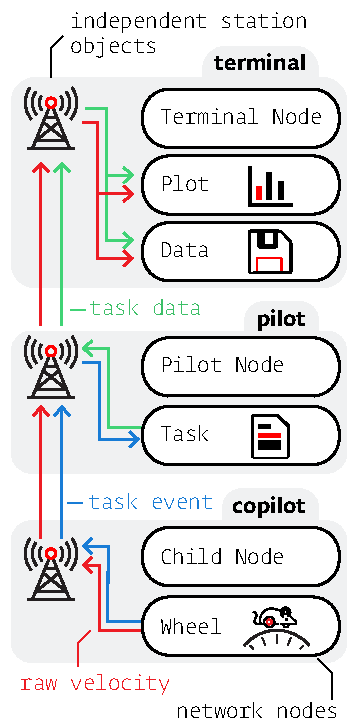
\includegraphics[]{figures/side_24_networking.pdf}
\caption{Autopilot segregates data streams efficiently---eg. raw velocity (red) can be plotted and saved by the terminal while only the task-relevant events (blue) are sent to the pilot. The pilot then sends trial-summarized data to the terminal (green).}
\label{fig:datastreams}
\end{marginfigure}

Both types of networking objects are tailored to their hosts by a set of callback functions --- \textbf{listens} --- that define how to handle each type of message. Messages have a uniform key-value structure, where the key indicates the listen used to process the message and the value is the message payload. This system makes adding new network-enabled components trivial:

\begin{pythoncode*}{label=A new networked LED}
class LED_RGB(Hardware):
    def __init__(self):
        # call self.color for a 'COLOR' message
        self.listens = {'COLOR': self.color}
        self.node = networking.Node(
            id      = 'BEST_LED',
            listens = self.listens)
        
    def color(msg):
        self.set_color(msg.value)
        
# elsewhere in the code, we change the color to red!
node.send(to='BEST_LED', key='COLOR', value=[255,0,0])
\end{pythoncode*}

\begin{marginfigure}[0cm]
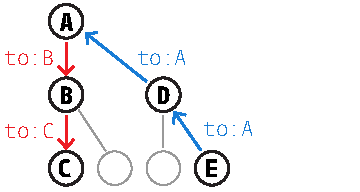
\includegraphics[]{figures/side_25_tree.pdf}
\caption{Treelike network structure---downstream messages are addressed by successive nodes, but upstream messages can always be pushed until the target is found.}
\label{fig:nettree}
\end{marginfigure}

Messages are serialized\sidenote{converted to binary suitable for sending between computers} with JSON\sidenote{though we have been investigating faster serialization libraries like \href{https://msgpack.org/}{msgpack}}, and can handle arrays, including on-the-fly compression with \href{https://www.blosc.org/}{blosc}. Net Nodes can create additional sockets to stream data that is stashed in a \href{https://docs.python.org/3/library/queue.html\#queue.Queue}{queue}, and can take advantage of message batching and compressing multiple arrays together when latency is less critical.

Network connectivity is currently treelike by default (Figure \ref{fig:nettree}) --- each independent networking object can have many children but at most one parent. This structure makes an implicit assumption about the anisotropy of information flow: `higher' nodes don't need to send messages to the `lowest' nodes, and the `lowest' nodes send all their messages to one or a few `higher' nodes. It enforces simplified delegation of responsibilities in both directions: a terminal shouldn't need to know about every hardware object connected to all of its connected pilots, it just sends messages to the pilots, who handle it from there. A far-downstream node shouldn't need to know exactly how to send its data back to the terminal, so it pushes it upstream until it reaches a node that does.

In the time since we released Autopilot it became clear that this treelike structure is useful for getting started quickly with the default full system configuration, but an unnecessary encumbrance for experimenting with different configurations. Alongside the \hyperref[sec:futureagents]{formalization} of the Agent classes, we intend to replace it with a peer-to-peer addressing system where every Autopilot has a unique ID and can message any other object in a given swarm with an \texttt{"agent:id"} address scheme. See \ref{future:network} for further discussion.

\clearpage
